\chapter{Simulation}
\label{chapter:Dokumentation-Simulation}

Bei dem Simulator handelt es sich um ein Java"=Programm, folglich wird er über den Aufruf

\texttt{\$ java Minimax}

gestartet.\footnote{Alternativ lassen sich die vier Konfigurationsdateien auch als Parameter übergeben, indem man sie der Reihe nach angibt:\\ \texttt{\$ java Minimax basis.txt erweiterung.txt steuerung.txt programm.txt}} Es öffnet sich daraufhin ein Dialog, in welchem man die benötigten Konfigurationsdateien angibt.

\begin{figure}[htb]
    \centering
    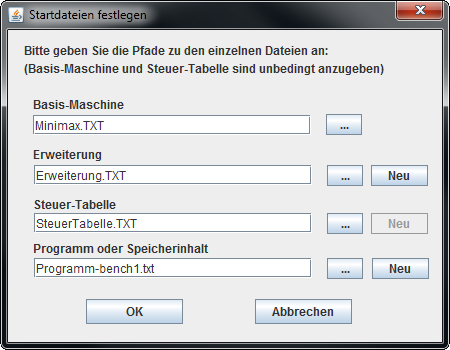
\includegraphics[width=0.7\textwidth]{dokumentation/res/minimax_load.png}
    \caption{Dialog zur Angabe der Konfigurationsdateien}
    \label{figure:Dokumentation-Simulation-Load}
\end{figure}

Nach Bestätigung öffnet sich das Kontrollfenster des Simulators. Um die Simulation zu starten, kann man entweder mit "`Ausführen $\rightarrow$ nächster Schritt"' (bzw. \texttt{Strg~+~Enter}) wählen oder man setzt mit "`Ausführen $\rightarrow$ Breakpoint setzen"' einen Breakpoint auf \texttt{END} und wählt anschließend "`Ausführen $\rightarrow$ bis Breakpoint ausführen"'. Dadurch läuft das Programm automatisch bis zum Ende durch und es muss nicht jeder Takt manuell bestätigt werden.

\begin{figure}[htb]
    \centering
    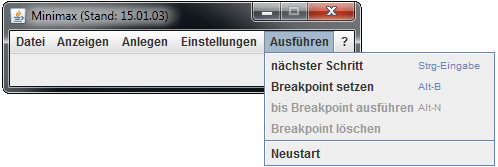
\includegraphics[width=0.7\textwidth]{dokumentation/res/minimax_run.png}
    \caption{Kontrollfenster des Simulators}
    \label{figure:Dokumentation-Simulation-Run}
\end{figure}

Die Konfiguration kann über das Datei"=Menü flexibel geändert werden. So können leicht unterschiedliche Speicherabbilder nacheinander geladen werden, ohne den Simulator neu starten zu müssen.

Hilfreiche Funktionen für die Analyse befinden sich im Menü "`Anzeigen"', z.B. die Anzeige des Speicherinhalts oder der Steuertabelle.

Weitere Informationen können dem Handbuch des Minimax"=Simulators \cite{minimax-handbuch} entnommen werden.